\section{ЭЛЕМЕНТЫ МАТЕМАТИЧЕСКОЙ ТЕОРИИ ИГР}

Во многих видах человеческой деятельности, а особенно в экономике, часто встречаются ситуации, в которых интересы различных лиц, организаций и т.д. противоречат друг  другу. Такие ситуации называют конфликтными. Например, при определении цен на товары интересы покупателя и продавца противоположны друг другу. Реальные конфликтные ситуации сложны для анализа, поэтому их нужно предварительно формализовать, отбросив все несущественные детали. Хорошей формой конфликтной ситуации, которая легко поддается формализации, является игра. Разрешение многих конфликтных ситуаций можно представить себе в виде игр, снабженных теми или иными правилами. Поэтому математическое моделирование игр является важной задачей.

Игры можно классифицировать по различным признакам, например, по количеству участников, по правилам распределения выигрышей и т.д.  Мы рассмотрим простейшие игры с двумя участниками, в которых выигрыш одного из игроков является проигрышем другого. Такие игры называются играми двух игроков с нулевой суммой.

Во всех играх присутствует понятие стратегии игры, т.е. описание поведения игрока в зависимости от сложившейся ситуации. Игроки могут применять различные стратегии с тем или иным успехом.

\subsection{Матричная игра двух игроков с нулевой суммой}

Мы рассмотрим следующую формализацию игры, которая состоит из двух наборов стратегий первого и второго игроков. При этом конкретное содержание стратегий  нас  интересовать не будет. Обозначим возможные стратегии первого игрока через \emph{A$_{1}$, А$_{2}$, ..., А$_{n}$}, а стратегии второго — \emph{В$_{1}$, В$_{2}$, ..., В$_{m}$}. Игра является одноходовой: первый игрок применяет одну из своих возможных стратегий, а второй отвечает стратегией из своего набора. После этого происходит распределение выигрышей, которое задается числами   — выигрышем первого игрока при условии, что он  применяет стратегию\emph{А$_{i}$}, а второй игрок отвечает стратегией \emph{В$_{j}$}. При этом выигрыш первого игрока является проигрышем второго. Числа   образуют матрицу, которую  называют матрицей выигрышей первого игрока или платежной матрицей. Величины \emph{a$_{ij}$}  могут быть как положительными, так и отрицательными или равными нулю. Если \emph{a$_{ij}$<0}, то первый игрок проигрывает, а второй выигрывает сумму, равную |\emph{a$_{ij}$}|.

\primer{Игра заключается в том, что первый игрок накрывает монету гербом или решкой вверх, а второй отгадывает. Если второй игрок угадывает, то получает выигрыш, равный 1.  Если второй игрок не угадывает, то он проигрывает 1. Возможные стратегии первого игрока: \emph{А$_{1}$} — накрыть монету гербом вверх, \emph{A$_{2}$} — накрыть монету решкой вверх. У второго игрока тоже две стратегии: \emph{В$_{1}$} — назвать орла, \emph{В$_{2}$} — назвать решку. Платежная матрица имеет следующий вид:}



\begin{table}[h!]
\label{table_4_1}
\begin{center}
\begin{tabular}{c|c|c}
 & \bfseries \emph{B$_{1}$} &\bfseries  \emph{B$_{2}$} \mdseries \\ \hline
\multicolumn{1}{c|}{\bfseries \emph{A$_{1}$} \mdseries} & -1 & 1 \\ \hline
\multicolumn{1}{c|}{\bfseries \emph{A$_{2}$}\mdseries}  & 1 & -1 \\ \hline
\end{tabular}
\end{center}
\end{table}

\subsection{Анализ игры в чистых стратегиях}

Основной задачей теории игр является выбор для игроков оптимальной в том или ином смысле стратегии. Платежную матрицу анализируют, стремясь найти такую стратегию, которая при любом поведении противника гарантировала бы достаточно высокий выигрыш. При этом считается, что противник ведет себя наиболее неблагоприятным образом.

\primer{Пусть матричная игра задается матрицей:}



\renewcommand{\arraystretch}{1.5}
\renewcommand{\tabcolsep}{0.3cm}
\begin{table}[h!]
\label{table_4_2}
\begin{center}
\begin{tabular}{c|c|c|c|c|c}
     &  \textbf{\emph{B$_{1}$}} &  \textbf{\emph{B$_{2}$}} & \textbf{\emph{B$_{3}$}} & \textbf{\emph{B$_{4}$}} &  \emph{$\alpha _{i}$} \\ \hline
 \multicolumn{1}{c|}{\textbf{\emph{A$_{1}$}}} & 10 & 7 & 4 & 1 & \fbox{1} \\ \hline
 \multicolumn{1}{c|}{\textbf{\emph{A$_{2}$}}} & 5 & -1 & 6 & 8 & -1 \\ \hline
 \multicolumn{1}{c|}{\textbf{\emph{A$_{3}$}}} & 2 & -8 & 5 & 3 & -8 \\ \hline
 \multicolumn{1}{c|}{\emph{$\beta_{j}$}} & 10 & 7 & \fbox{6} & 8 & \diagbox{6}{1} \\
\end{tabular}
\end{center}
\end{table}






При наиболее неблагоприятном поведении второго игрока стратегия \emph{A$_{1}$} первого игрока доставляет ему минимальный гарантированный выигрыш 1. Стратегии \emph{A$_{2}$} и \emph{A$_{3}$} в этом смысле хуже, чем \emph{A$_{1}$}, так как при неблагоприятных условиях ведут к проигрышу. С точки зрения второго игрока наилучшей является стратегия \emph{B$_{3}$}, так как ее применение может привести к проигрышу 6, а при остальных стратегиях можно проиграть больше. В этом смысле \emph{A$_{1}$} наилучшая стратегия первого, а \emph{B$_{3}$} — второго игрока.

В общем случае игроки оценивают свои стратегии следующим образом. Первый игрок, рассматривая свои стратегии, ищет $\min\limits_{j}$ \emph{a$_{ij}$}, а затем выбирает такую стратегию \emph{A$_{i}$}, при которой эта величина наибольшая. При этом он вычисляет величину
\begin{equation}
\label{equation_4_1}
\alpha = \max_{i} \min_{j} \emph{a$_{ij}$}
\end{equation}

Величина $\alpha$ называется \emph{нижней ценой игры}, а правило выбора наилучшей стратегии называется \emph{правилом максимина}. В нашем примере $\alpha$=1. Второй игрок находит $\max\limits_{i}$ \emph{a$_{ij}$}, затем выбирает стратегию, при которой эта величина наименьшая, то есть он вычисляет величину  $\beta$ = $\min\limits_{i} \max\limits_{j} \emph{a$_{ij}$}$. $\beta$ называется \emph{верхней ценой игры}, а правило, которым пользуется второй игрок для выбора своей наилучшей стратегии, — \emph{правилом минимакса}. В нашем примере $\beta$ = 6. Можно доказать, что для любой платежной матрицы $\alpha \leqslant \beta$

В рассмотренном примере большую роль  играет  информация  о  ходе противника. Если второй игрок знает, что первый применит стратегию \emph{A$_{1}$}, он может, выбирая стратегию \emph{B$_{4}$} уменьшить свой проигрыш по сравнению со стратегией \emph{B$_{3}$}. Если первый знает, что второй применит стратегию \emph{B$_{3}$}, он имеет возможность увеличить свой выигрыш, применяя стратегию \emph{A$_{2}$}. То есть приведенная выше оценка качества стратегий теряет смысл при наличии информации о поведении противника. Такая ситуация характерна для большинства игр. Информация о поведении противника — залог успеха в игре. Однако для некоторых платежных матриц это не так.

\primer{Пусть игра задаётся матрицей}


%\renewcommand{\arraystretch}{1.5}
%\renewcommand{\tabcolsep}{0.3cm}
\begin{table}[h!]
\label{table_4_3}
\begin{center}
\begin{tabular}{c|c|c|c|c|c|}
     &  \textbf{\emph{B$_{1}$}} &  \textbf{\emph{B$_{2}$}} & \textbf{\emph{B$_{3}$}} & \textbf{\emph{B$_{4}$}} &  \emph{$\alpha _{i}$} \\ \hline
  \multicolumn{1}{c|}{\textbf{\emph{A$_{1}$}}} & 2 & 4 & 7 & 5 & 2 \\ \hline
  \multicolumn{1}{c|}{\textbf{\emph{A$_{2}$}}} & 7 & 6 & 8 & 7 & \fbox{6} \\ \hline
  \multicolumn{1}{c|}{\textbf{\emph{A$_{3}$}}} & 5 & 3 & 4 & 1 & 1 \\ \hline
  \multicolumn{1}{c|}{\emph{$\beta_{j}$}} & 7 & \fbox{6} & 8 & 7 &   \\
\end{tabular}
\end{center}
\end{table}


В этом примере верхняя и нижняя цены игры совпадают $\alpha = \beta = 6$. Если первый игрок придерживается стратегии \emph{A$_{2}$}, второму ничего не остается, как выбрать стратегию \emph{B$_{2}$}, иначе он проиграет больше. Если  второй игрок придерживается стратегии \emph{B$_{2}$}, то первому нужно придерживаться стратегии \emph{A$_{2}$}, иначе он выиграет меньше. Пара стратегий \emph{A$_{2}$}, \emph{B$_{2}$} является парой оптимальных стратегий для обоих игроков, и информация о поведении противника здесь роли не играет.

В случае, когда верхняя и нижняя цены игры совпадают, говорят, что игра имеет седловую точку в \emph{чистых стратегиях}. В этом случае всегда найдется такой элемент \emph{a$_{i_{0}j_{0}}$}  платежной матрицы,  который удовлетворяет неравенствам
\begin{equation}
\label{equation_4_2}
\emph{a$_{ij_{0}}$} \leqslant \emph{a$_{i_{0}j_{0}}$} \leqslant \emph{a$_{i_{0}j}$}
\end{equation}
при любых \emph{i, j}. Этот элемент \emph{a$_{i_{0}j_{0}}$} называется \emph{седловой точкой игры,} а стратегии \emph{A$_{i_{0}}$}, \emph{B$_{j_{0}}$} называют \emph{оптимальными стратегиями,} отвечающими седловой точке. Слова “чистая стратегия” означают просто стратегии первого и второго  игроков. Существование  седловой точки является исключением. Большинство игр не имеет седловой точки в чистых стратегиях.  Если  же игра имеет седловую точку, то она практически теряет смысл, так как ходы противников предрешены. Часто говорят, что в этом случае игра решается в чистых стратегиях,  а пару оптимальных стратегий называют решением игры в чистых стратегиях.

\subsection{Понятие смешанной стратегии. Седловая точка игры
в смешанных стратегиях}

Предположим, что игра повторяется много раз, то есть, проводится достаточно длинная серия партий, и каждый из игроков выбирает в каждой партии свою чистую стратегию случайным образом, в соответствии с некоторыми вероятностями выбора стратегий.

\opredelenie{\emph{Смешанной стратегией игрока называется совокупность вероятностей выбора им своих чистых стратегий.}}

Обозначим через  \emph{р$_{1}$, р$_{2}$, ... , р$_{n}$}  вероятности выбора чистых стратегий первым игроком в серии партий. Эта совокупность чисел и составляет смешанную стратегию первого игрока.  Смешанная стратегия — это \emph{n}-мерный вектор, компоненты которого удовлетворяют условиям
\begin{equation}
\label{equation_4_3}
p_{i} \geqslant 0 \; (i = 1, 2, ..., n); \; p_{1} + p_{2} + ... + p_{n} = 1.
\end{equation}

Под смешанной стратегией второго игрока будем понимать любой \emph{m}-мерный вектор {$q_{1}, q_{2}, ..., q_{m},$} удовлетворяющий условиям
\begin{equation}
\label{equation_4_4}
q_{i} \geqslant 0 \; (i = 1, 2, ..., m); \; q_{1} + q_{2} + ... + q_{m} = 1.
\end{equation}

\opredelenie{\emph{Средним выигрышем первого игрока или платежной функцией игры называется функция n+m переменных} $M(\vec{p}, \vec{q}) = \sum\limits_{i, j} a_{ij} p_{i} q_{j}$ \emph{определенная на смешанных стратегиях первого и второго игроков.}}

При конкретном выборе смешанных стратегий $M(\vec{p}, \vec{q})$   является математическим ожиданием выигрыша первого игрока.

\opredelenie{\emph{Седловой точкой игры в смешанных стратегиях называется такая пара смешанных стратегий первого и второго игроков}}
\begin{equation}
\label{equation_4_5}
    {\vec{p}^0} = \{p_{1}^0, p_{2}^0, ..., p_{n}^0\}; \; {\vec{q}^0} = \{q_{1}^0, q_{2}^0, ..., q_{m}^0\},
\end{equation}
\emph{для которой при любых смешанных стратегиях $\vec{p}, \vec{q}$ выполняются неравенства}
\begin{equation}
\label{equation_4_6}
M(\vec{p}^0, \vec{q}^0) \leqslant M(\vec{p}^0, \vec{q}^0) \leqslant M(\vec{p}^0, \vec{q})
\end{equation}

Седловая точка представляет собой наиболее выгодную пару смешанных стратегий для каждого игрока, так как отступление от нее невыгодно им обоим.

Отметим, что чистые стратегии можно рассматривать как частный случай смешанных. Например, стратегию А1 первого игрока можно рассматривать как смешанную стратегию \{1, 0, 0, ...,0\}.

\primer{Составим платежную функцию игры в так называемое тюремное очко. Каждый из игроков выбрасывает определенное число пальцев (1, 2 или 3). Если сумма выброшенных пальцев четная, то выигрывает первый игрок и его выигрыш равен сумме выброшенных пальцев. Если сумма нечетная, выигрывает второй игрок и его выигрыш равен выброшенной сумме. Здесь каждый из игроков имеет по три стратегии и легко составить платежную матрицу}
\renewcommand{\arraystretch}{1.5}
\renewcommand{\tabcolsep}{0.2cm}
\begin{table}[h!]
\label{table_4_4}
\begin{center}
\begin{tabular}{c|c|c|c}
     &  \textbf{\emph{B$_{1}$}} &  \textbf{\emph{B$_{2}$}} & \textbf{\emph{B$_{3}$}}  \\ \hline
   \multicolumn{1}{c|}{\textbf{\emph{A$_{1}$}}} & 2 & -3 & 4  \\ \hline
   \multicolumn{1}{c|}{\textbf{\emph{A$_{2}$}}} & -3 & 4 & -5  \\ \hline
   \multicolumn{1}{c|}{\textbf{\emph{A$_{3}$}}} & 4 & -5 & 6 \\
\end{tabular}
\end{center}
\end{table}

Если игра повторяется много раз и чистые стратегии выбираются в  соответствии с вероятностями  \{\emph{р$_{1}$, р$_{2}$, р$_{3}$}\} для первого игрока и  \{\emph{q$_{1}$, q$_{2}$, q$_{3}$}\} для второго, то платежная функция этой игры имеет вид
\begin{equation}
\label{equation_4_7}
M(\vec{p}, \vec{q}) = 2p_{1}q_{1} - 3p_{1}q_{2} + 4p_{1}q_{3} - 3p_{2}q_{1} + 4p_{2}q_{2} - 5p_{2}q_{3} + 4p_{3}q_{1} - 5p_{3}q_{2} + 6p_{3}q_{3}.
\end{equation}

Посчитаем значение платежной функции при следующих смешанных стратегиях $\vec{p}^0$ = \Large \{$\frac{1}{4}; \frac{1}{2}; \frac{1}{4}$\}, \normalsize $\; \vec{q}^0$ = \Large \{$\frac{1}{4}; \frac{1}{2}; \frac{1}{4}$\} \normalsize, $M(\vec{p}^0, \vec{q}^0)$ = 0.

Можно показать, что пара стратегий $\vec{p}^0$, $\vec{q}^0$ в этом примере является седловой точкой.

\subsection{Теорема Фон-Неймана. Нахождение седловой точки игры
 в смешанных стратегиях}

Следующая теорема доказана американским математиком Фон-Нейманом (см., например, \cite{literature_neiman}).

\teorema{\emph{Для каждой матричной игры двух игроков с нулевой суммой существует пара смешанных стратегий игроков, которая является седловой точкой игры в смешанных стратегиях.}}

Теорема утверждает существование седловой точки, но вовсе не ее единственность. В некоторых случаях игра может иметь бесчисленное множество седловых точек в смешанных стратегиях.

Нахождение седловой точки в смешанных стратегиях называют \emph{решением игры} в смешанных стратегиях. Решение игры сводится к решению пары двойственных задач линейного программирования. Сформулируем эту пару задач.

\emph{Для первого игрока смешанная стратегия в том и только в том случае отвечает седловой точке в смешанных стратегиях, когда она является точкой максимума задачи}

\begin{equation}
\label{equation_4_8}
A) \; z = \nu \to \max
\end{equation}
\begin{equation}
\label{equation_4_9}
\begin{cases}
a_{11}p_{1} + a_{21}p_{2} + ... + a_{n1}p_{n} \leqslant \nu,\\
a_{12}p_{1} + a_{22}p_{2} + ... + a_{n2}p_{n} \leqslant \nu, \\
................................................. \\
a_{1m}p_{1} + a_{2m}p_{2} + ... + a_{nm}p_{n} \leqslant \nu; \\
p_{1} + p_{2} + ... + p_{n} = 1; \\
\end{cases}
\end{equation}



Здесь $\nu$ — независимая переменная, которая, вообще говоря, не подчиняется условию неотрицательности.

\emph{Для второго игрока смешанная стратегия $q_{1}^0, q_{2}^0, ..., q_{m}^0$   в том и только в том случае отвечает седловой точке, когда она является точкой минимума задачи}
\begin{equation}
\label{equation_4_10}
B) \; f = u \to \min
\end{equation}
\begin{equation}
\label{equation_4_11}
\begin{cases}
a_{11}q_{1} + a_{12}q_{2} + ... + a_{1m}q_{m} \leqslant u, \\
a_{21}q_{1} + a_{22}q_{2} + ... + a_{2m}q_{m} \leqslant u, \\
............................................ \; \; q_{i} \geqslant 0 (i = \overline{1, m}) \\
a_{n1}q_{1} + a_{n2}q_{2} + ... + a_{nm}q_{m} \leqslant u, \\
q{1} + q_{2} + ... + q_{m} = 1; \\
\end{cases}
\end{equation}


Здесь переменная \emph{u} не подчинена условию неотрицательности.

Форму этих задач линейного программирования нетрудно объяснить. Пусть $\nu$ — оптимальный выигрыш первого игрока. Оценивая свою смешанную стратегию \emph{$\{$р$_{1}$, р$_{2}$, ... , р$_{n}\}$,} первый игрок стремится, чтобы при каждой чистой стратегии второго игрока его средний выигрыш был не меньше оптимального. Если второй игрок применяет свою стратегию \emph{В$_{j}$,} то первый должен выбирать смешанную стратегию, удовлетворяющей неравенству
\begin{equation}
\label{equation_4_12}
a_{1j}p_{1} + a_{2j}p_{2} + ... + a_{nj}p_{n} \geqslant \nu, \; j = 1, 2, ..., m.
\end{equation}

Аналогично рассуждает и второй игрок. Если \emph{u} — проигрыш второго игрока, который он стремится минимизировать, то оценивая свою смешанную стратегию \emph{$\{$q$_{1}$, q$_{2}$, ... , q$_{m}\}$,} второй игрок должен стремиться к выполнению неравенств
\begin{equation}
\label{equation_4_13}
a_{i1}q_{1} + a_{i2}q_{2} + ... + a_{im}q_{m} \leqslant u, \; i = 1, 2, ..., n.
\end{equation}

Задачи A) и В) двойственны друг другу. Решение их в общем случае громоздко. Но для игр размера 2 $\times$ \emph{m} и \emph{n} $\times$ 2 одну из задач можно решить графически, а решение другой найти с помощью условий дополнительной нежесткости. Кроме того, в общем случае можно так преобразовать задачи А) и В), что они могут быть решены двойственным симплекс-методом в форме, которая рассматривалась выше.

\subsection{Графическое решение игр размера 2 $\times$ \emph{m} и \emph{n} $\times$ 2}

Рассмотрим игру размера 2 $\times$ \emph{m}. Для оптимальной стратегии первого игрока имеем задачу
\begin{equation}
\label{equation_4_14}
z = \nu \to \max;
\end{equation}
\begin{equation}
\label{equation_4_15}
\begin{cases}
a_{11}p_{1} + a_{21}p_{2} \geqslant \nu, \\
a_{12}p_{1} + a_{22}p_{2} \geqslant \nu, \\
.......................... \\
a_{1m}p_{1} + a_{2m}p_{2} \geqslant \nu, \\
p{1} + p_{2} = 1; \; p_{1}, p_{2} \geqslant 0 \\
\end{cases}
\end{equation}


Поскольку \emph{p$_{2}$ = 1 - p$_{1}$,} то, подставляя это выражение вместо \emph{p$_{2}$} в остальные ограничения, получим задачу с двумя переменными \emph{p$_{1}$} и $\nu$
\begin{equation}
\label{equation_4_16}
z = \nu \to \max;
\end{equation}
\begin{equation}
\label{equation_4_17}
\begin{cases}
(a_{11} - a_{21})p_{1} + a_{21} - \nu \geqslant 0,  \\
(a_{12} - a_{22})p_{1} + a_{22} - \nu \geqslant 0,  \\
.......................... \\
(a_{1m} - a_{2m})p_{1} + a_{2m} - \nu \geqslant 0;  \\
0 \leqslant p_{1} \leqslant 1. \\
\end{cases}
\end{equation}


Эту задачу можно решать графически. Для задач размером \emph{n} $\times$ 2 точно также преобразуется задача для второго игрока
\begin{equation}
\label{equation_4_18}
f = u \to \min;
\end{equation}
\begin{equation}
\label{equation_4_19}
\begin{cases}
a_{11}q_{1} + a_{12}q_{2} \leqslant u,  \\
a_{21}q_{1} + a_{22}q_{2} \leqslant u,  \\
.......................... \\
a_{n1}q_{1} + a_{n2}q_{2} \leqslant u,  \\
q_{1} + q_{2} = 1; \; q_{1}, q_{2} \geqslant 0. \\
\end{cases}
\end{equation}


\primer{Решить игру с платежной матрицей}

\renewcommand{\arraystretch}{1.5}
\renewcommand{\tabcolsep}{0.2cm}
\begin{table}[h!]
\label{table_4_5}
\begin{center}
\begin{tabular}{|c|c|c|c|c|}
    \hline
     &  \textbf{\emph{B$_{1}$}} &  \textbf{\emph{B$_{2}$}} & \textbf{\emph{B$_{3}$}} & \textbf{\emph{B$_{4}$}}  \\ \hline
  \multicolumn{1}{|c|}{\textbf{\emph{A$_{1}$}}} & 2 & 1 & 5 & 3  \\ \hline
  \multicolumn{1}{|c|}{\textbf{\emph{A$_{2}$}}} & 1 & 3 & 4 & 0,5 \\ \hline
\end{tabular}
\end{center}
\end{table}


Соответствующая задача линейного программирования имеет вид:
\begin{equation}
\label{equation_4_20}
z = \nu \to \max;
\end{equation}
\begin{equation}
\label{equation_4_21}
\begin{aligned}
q_1\\
q_2\\
q_3\\
q_4\\
u\\
\end{aligned}
\left\{
\begin{aligned}
&2p_1 + p_2 \geqslant \nu \\
&p_1 + 3p_2 \geqslant \nu \\
&5p_1 + 4p_2 \geqslant \nu \\
&3p_1 + 0,5p_2 \geqslant \nu \\
&p_1 + p_2 = 1 \\
\end{aligned}
\right.
\end{equation}
\begin{equation}
\label{equation_4_22}
p_1, p_2 \geqslant 0
\end{equation}
Исключим переменную \emph{p$_{2}$; p$_{2}$=1-p$_{1}$} :













\begin{equation}
\label{equation_4_23}
z=\nu \to max;
\end{equation}
\begin{equation}
\label{equation_4_24}
   \begin{cases}
p_1-\nu \geqslant -1, \\
-2p_1-\nu \geqslant -3, \\
p_1-\nu \geqslant -4, \\
2,5p_1-\nu\geqslant -0,5; \\
    \end{cases}
\end{equation}
\begin{equation}
\label{equation_4_25}
    0 \leqslant p_1 \leqslant 1.
\end{equation}
Полученную задачу решаем графически (рис. 4.1).
\begin{figure}[!h]
\center{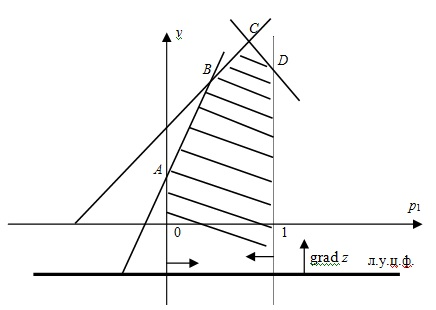
\includegraphics{pictures/picturefile_4_1.jpg}}
\caption*{Рис. 4.1. Графическое решение задачи примера 4.5}
\label{fig:image}
\end{figure}

Точкой максимума является точка \emph{C}, удовлетворяющая системе уравнений
\begin{equation}
\label{equation_4_26}
    \begin{cases}
    p_1-\nu=-1,  \\
    2p_1+\nu=3.  \\
    \end{cases}
\end{equation}

Отсюда $p_1^0=\frac{2}{3}; p_2^0=\frac{1}{3}$ — смешанная стратегия первого игрока в седловой точке.  Для нахождения смешанной стратегии второго игрока применим условия  дополнительной нежесткости. Двойственная задача имеет вид
\begin{equation}
\label{equation_4_27}
    f=u \to min;
\end{equation}
\begin{equation}
\label{equation_4_28}
\begin{aligned}
p_1\\
p_2\\
\nu \\
\end{aligned}
\left\{
\begin{aligned}
&2q_1 + q_2 + 5q_3 + 3q_4 \leqslant u, \\
&q_1 + 3q_2 + 4q_3 + 0,5q_4 \leqslant u, \\
&q_1 + q_2 + q_3 + q_4 = 1; \\
\end{aligned}
\right.
\end{equation}

\begin{equation}
\label{equation_4_29}
    q_1, q_2, q_3, q_4 \geqslant 0.
\end{equation}

Условия дополнительной нежесткости запишутся так:

\begin{equation}
\label{equation_4_30}
\begin{cases}
p_1^0 (2q_1^0 + q_2^0 + 5q_3^0 + 3q_4^0 - u^0) = 0, \\
p_2^0 (q_1^0 + 3q_2^0 + 4q_3^0 + 0,5q_4^0 - u^0) = 0, \\
\nu^0 (q_1^0 + q_2^0 + q_3^0 + q_4^0 - 1) = 0,\\
q_1^0 (2p_1^0 + p_2^0 - \nu^0) = 0,\\
q_2^0 (p_1^0 + 3p_2^0 - \nu^0) = 0,\\
q_3^0 (5p_1^0 + 4p_2^0 - \nu^0) = 0,\\
q_4^0 (3p_1^0 + 0,5p_2^0 - \nu^0) = 0,\\
u_1^0 (p_1^0 + p_2^0 - 1) = 0.\\
\end{cases}
\end{equation}

Подставим найденные $p_1^0=\frac{2}{3}$ и $p_2^0=\frac{1}{3}$ в эти равенства, учитывая, что $\nu^0 = u^0 = \frac{5}{3}.$ Четвертое, пятое и восьмое равенства будут тождествами. Из шестого и седьмого следует, что $q_3^0  q_4^0 = 0.$ Для определения $q_1^0$ и $q_2^0$ имеем

\begin{equation}
\label{equation_4_31}
    \begin{cases}
    2q_1^0 + q_2^0 = \frac{5}{3},  \\
    q_1^0 + 3q_2^0 = \frac{5}{3}.  \\
    \end{cases}
\end{equation}

Откуда следует $q_1^0 = \frac{2}{3}; q_2^0 = \frac{1}{3}.$ Таким образом, седловая точка игры
\begin{equation}
\label{equation_4_32}
   \vec{p}^0 = \large \{\frac{2}{3}; \frac{1}{3}\} \normalsize;  \vec{q}^0 = \large \{\frac{2}{3}; \frac{1}{3}; 0; 0\} \normalsize.
\end{equation}

Отметим, что средний выигрыш в седловой точке называется обычно \emph{ценой игры} в смешанных стратегиях. В нашей паре двойственных задач для первого и второго играков цена игры равна $\nu^0 = u^0$ В примере 4.5 цена игры равна 5/3.
\subsection{Решение игры двойственным симплекс-методом}

Преобразуем пару двойственных задач \emph{А)} и \emph{В)} так, чтобы удобно было применять  двойственный симплекс-метод. Прежде всего, отметим, что седловая точка игры не изменится, если ко всем элементам платежной матрицы прибавить одну и ту же константу. Действительно, если ко всем элементам прибавить константу С, то мы получим новую платежную функцию
\begin{equation}
\label{equation_4_33}
M_{1}(\vec{p}, \vec{q}) = \sum\limits_{i, j}(a_{i,j}+C)p_{i}q_{j} =
\sum\limits_{i, j}a_{i,j}p_{i}q_{j}+C\left(\sum\limits_{i, j}p_{i}q_{j}\right)=M(\vec{p}, \vec{q})+C.
\end{equation}

Таким образом, новая платежная функция отличается от старой постоянным слагаемым \emph{C}. Если $\{{\vec{p}^0, \vec{q}^0}\}$ - седловая точка старой платежной функции, то
\begin{equation}
\label{equation_4_34}
M(\vec{p}, \vec{q}^0) \leqslant M(\vec{p}^0, \vec{q}^0) \leqslant M(\vec{p}^0, \vec{q}).
\end{equation}

Прибавляя к обеим частям каждого этих неравенств константу \emph{C}, получим
\begin{equation}
\label{equation_4_35}
M_1(\vec{p}, \vec{q}^0) \leqslant M_1(\vec{p}^0, \vec{q}^0) \leqslant M_1(\vec{p}^0, \vec{q}).
\end{equation}

То есть $\{{\vec{p}^0, \vec{q}^0}\}$ является седловой точкой и новой платежной функции. Прибавляя константу \emph{C} ко всем элементам матрицы мы всегда можем добиться того, чтобы цена игры была положительна, а седловая точка осталась бы прежней. При этом, поскольку в решениях задач \emph{А)} и \emph{В)} ${u^0}$ и ${v^0}$  положительны, можно считать переменные подчиненными дополнительным условиям ${v>0}$ ; ${u>0}$, которые на
точки оптимума задач не повлияют.

Рассмотрим ограничение $p_1+p_2+...+p_n=1$ и разделим обе его части на \emph{v}, обозначив $\frac{p_i}{v}=x_{i} (i=1,2,...,n).$ Поскольку в нашей задаче $v \to max$ мы получим задачу на минимум для новой целевой функции
\begin{equation}
\label{equation_4_36}
    z_1=\frac{1}{v}=x_1+x_2+...+x_n \to min.
\end{equation}

Разделив все  неравенства  системы  ограничений задачи \emph{А)} на \emph{v}, получим для переменных $x_i$ условия
\begin{equation}
\label{equation_4_37}
\left\{
\begin{array}{l}
a_{11}x_1+a_{21}x_2+...+a_{n1}x_n \geqslant 1,\\
a_{12}x_1+a_{22}x_2+...+a_{n2}x_n \geqslant 1,\\
..................................................\\
a_{1m}x_1+a_{2m}x_2+...+a_{nm}x_n \geqslant 1;\\
\end{array}
\right.
\end{equation}
\begin{equation}
\label{equation_4_38}
    x_i \geqslant 0, i=\overline{1,n}.
\end{equation}
Производя аналогичные преобразования задачи \emph{В)} и вводя новые переменные $y_j=\frac{q_j}{u},$ получаем новую задачу:
\begin{equation}
\label{equation_4_39}
    f_1=\frac{1}{u}=y_1+y_2+...+y_m \to max
\end{equation}
\begin{equation}
\label{equation_4_40}
\left\{
\begin{array}{l}
a_{11}y_1+a_{12}y_2+...+a_{1m}y_m \leqslant 1,\\
a_{21}y_1+a_{22}y_2+...+a_{2m}y_m \leqslant 1,\\
..................................................\\
a_{n1}y_1+a_{n2}y_2+...+a_{nm}y_m \leqslant 1;\\
\end{array}
\right.
\end{equation}
\begin{equation}
\label{equation_4_41}
    y_i \geqslant 0, i=\overline{1,m}.
\end{equation}

Мы получили пару симметрично-двойственных задач. Последнюю задачу можно решать симплекс-методом непосредственно после уравнивания неравенств, а решение другой можно будет прочесть по последней симплекс-таблице. Если $y_1^0,y_2^0,...,y_m^0$ - точка максимума задачи для второго игрока, то вероятности чистых стратегий в седловой точке можно найти по формулам
\begin{equation}
\label{equation_4_42}
        q_1^0=\frac{y_1^0}{f_{1max}}; q_2^0=\frac{y_2^0}{f_{1max}};...; q_m^0=\frac{y_m^0}{f_{1max}}
\end{equation}

Если $x_1^0, x_2^0,...,x_n^0$  — точка минимума задачи для первого игрока, то вероятности стратегий в седловой точке равны
\begin{equation}
\label{equation_4_43}
    p_1^0=\frac{x_1^0}{z_{1min}}; p_2^0=\frac{x_2^0}{z_{1min}};...;p_m^0=\frac{x_m^0}{z_{1min}}.
\end{equation}

Отметим, что $f_{min}=z_{max}=A.$ Цена игры при этом равна $A-C$, где \emph{С} — константа, которую мы прибавляли, гарантируя неравенства $v>0; u>0.$

\primer{Наметим нахождение седловой точки в смешанных стратегиях для игры примера 4.4. Прибавим ко всем элементам матрицы число 6. Получим матрицу
$$
\bordermatrix{
         & y_1 & y_2 & y_3 \cr
     x_1 &  8  &  3  & 10  \cr
     x_2 &  3  & 10  & 1   \cr
     x_3 & 10  &  1  & 12  \cr }
$$

Построим пару двойственных задач в переменных $x_1, x_2, x_3$ и $y_1, y_2, y_3.$

\begin{center}
\begin{minipage}
  {0.4\textwidth}
$1) z_1 = x_1 + x_2 + x_3 \to min;$
$$
\left\{
\begin{array}{l}
8x_1 + 3x_2 + 10x_3 \geqslant 1,\\
3x_1 + 10x_2 + x_3 \geqslant 1,\\
10x_1 + x_2 + 12x_3 \geqslant 1;\\
\end{array}
\right.
$$
$x_1, x_2, x_3 \geqslant 0.$
\end{minipage}
 \hfill
 \begin{minipage}
 {0.4\textwidth}
$2) f_1 = y_1 + y_2 + y_3 \to max;$
$$
\left\{
\begin{array}{l}
8y_1 + 3y_2 + 10y_3 \leqslant 1,\\
3y_1 + 10y_2 + y_3 \leqslant 1,\\
10y_1 + y_2 + 12y_3 \leqslant 1;\\
\end{array}
\right.
$$
$y_1, y_2, y_3 \geqslant 0.$
\end{minipage}
\end{center}

Вторую задачу можно решить симплекс-методом непосредственно после уравнивания неравенств системы ограничений.}
\subsection{Доминирование и дублирование стратегий. Упрощение игры}

Если платежная матрица такова, что каждый элемент некоторой строки с номером \emph{i} не меньше соответствующего элемента строки с номером \emph{k} и, по меньшей мере, один ее элемент строго больше соответствующего элемента строки с номером \emph{k}, то говорят, что стратегия $A_i$ первого  игрока  доминирует над его стратегией $A_k.$ Очевидно, что стратегия первого игрока, для которой есть доминирующая, не может быть оптимальной чистой стратегией для него, или входить в его оптимальную смешанную стратегию с ненулевой вероятностью. Таким образом, такую стратегию можно исключить из рассмотрения, вычеркнув из матрицы строку с номером \emph{k}. Аналогично, если каждый элемент столбца с номером \emph{j} платежной матрицы не больше соответствующего элемента столбца с номером \emph{r} и, по меньшей мере, один его элемент строго меньше соответствующего элемента столбца с номером \emph{r}, то говорят, что стратегия $B_j$ второго игрока доминирует над его стратегией $B_r.$ При поиске оптимальных стратегий столбец с номером \emph{r} можно вычеркнуть.

Вообще говоря, в платежной матрице могут быть одинаковые строки или столбцы. Соответствующие стратегии называются дублирующими. Очевидно, что дублирующие стратегии целесообразно отбросить.

Выявление доминирующих и дублирующих стратегий позволяет произвести упрощение игры, то есть сократить размеры ее платежной матрицы, исходя из того очевидного факта, что стратегии, над которыми есть доминирующие, применяться в игре не будут, а избавиться от дублирования стратегий можно в виду их полной взаимозаменяемости. Упрощение игры обычно производят в следующем порядке. Вначале с точки зрения первого игрока выявляют его стратегии, над которыми есть доминирующие, а также его дублирующие стратегии. Соответствующие строки платежной матрицы вычеркивают. Для сокращенной матрицы проделывают то же самое, но с точки зрения второго игрока. Упрощение игры считается завершенным, если на очередном шаге в платежной матрице будут отсутствовать доминирующие и дублирующие стратегии для первого и второго игроков.

\zamechanie{\textit{Если исходная платежная матрица имеет седловую точку в чистых стратегиях, то процесс упрощения игры приведет к матрице размера $1\times 1$, состоящей из одного элемента (седловой точки).}}

\primer{Рассмотрим игру с платежной матрицей

\begin{center}
  $
    \begin{pmatrix}
      2 & 4 & 7 & 5 \\
      7 & 6 & 8 & 7 \\
      5 & 3 & 4 & 1 \\
      7 & 6 & 0 & 9 \\
  \end{pmatrix}
  $
\end{center}

Нетрудно видеть, что стратегия первого игрока $A_2$ доминирует над стратегиями $A_1$ и $A_3$, которые можно отбросить. В оставшейся матрице с точки зрения второго игрока стратегия $B_2$ доминирует над стратегиями $B_1$ и $B_4$. Отбрасывая последние две стратегии, получим упрощенную игру

\begin{table}[h!]
\label{table_4_6}
\begin{center}
\begin{tabular}[t]{|p{1.5em}|p{1.5em}|p{1.5em}|}
    \hline
     {} &  \textbf{\emph{B$_{2}$}} & \textbf{\emph{B$_{3}$}} \\ \hline
   \multicolumn{1}{|c|} {\textbf{\emph{A$_{2}$}}} & 6 & 8\\ \hline
   \multicolumn{1}{|c|} {\textbf{\emph{A$_{4}$}}} & 6 & 0\\ \hline
\end{tabular}
\end{center}
\end{table}

Возвращаясь на точку зрения первого игрока, мы видим, что в последней игре стратегия $A_2$ доминирует над стратегией $A_4$. Отбрасывая последнюю стратегию и сравнивая оставшиеся стратегии второго игрока, приходим к выводу, что стратегия $B_3$ должна быть отброшена. Получилась игра размера $1\times 1$ и седловая точка $(A_2, B_2)$ в чистых стратегиях.}
\subsection{Типичный пример применения теории игр в экономике}

Пусть предприятие  может выпускать три вида продукции: \emph{А}, \emph{B} и \emph{C}. Прибыль от реализации продукции зависит от уровня спроса, о котором ничего неизвестно, но он принимает три возможных значения. Прибыль от реализации каждого изделия вида \emph{А}, \emph{B} или \emph{C} в зависимости от уровня спроса представлена в таблице:
\begin{table}[h!]
\label{table_4_7}
\begin{center}
\begin{tabular}[t]{|p{12.8em}|p{1em}|p{1em}|p{1em}|}
\hline
   \textbf{\diagbox{Продукция}{Спрос}}  &  \textbf{I} &  \textbf{II} & \textbf{III}\\ \hline
   \multicolumn{1}{|c|} {\textbf{\emph{A}}} & 8 & 3 & 10 \\ \hline
   \multicolumn{1}{|c|} {\textbf{\emph{B}}} & 3 & 10 & 1 \\ \hline
   \multicolumn{1}{|c|} {\textbf{\emph{C}}} & 10 & 1 & 12 \\ \hline
\end{tabular}
\end{center}
\end{table}

Эту ситуацию можно рассматривать как игру двух игроков, если предприятие будет считать, что спрос ведет себя самым невыгодным для него образом. Рассматривая соответствующую игру в смешанных стратегиях, нетрудно найти седловую точку, в которой вероятности стратегий $p_1^0, p_2^0, p_3^0$ первого игрока (предприятия) укажут удельные веса каждого вида продукции,  которые обеспечат предприятию оптимальную гарантированную прибыль при самом неблагоприятном поведении спроса. Игры, подобные рассмотренной, носят название \emph{игр с природой}. Решение в рамках матричной игры с нулевой суммой позволяет принимать решения, являющиеся наилучшими при самых неблагоприятных условиях. Однако при более благоприятных условиях это решение может оказаться далеко не лучшим.
\subsection{Другие разновидности игр}

В настоящее время теория игр является довольно развитым разделом математики, содержащим различные обобщения матричных игр с нулевой суммой. Рассмотрим кратко основные направления таких обобщений. Отказ от абсолютной противоположности интересов игроков (от антагонистичности игры) приводит к неантагонистическим играм, простейшими из которых являются \emph{биматричные игры.} Биматричной игрой называется  игра  двух игроков  с  ненулевой  суммой,  в которой выигрыши задаются двумя матрицами отдельно для каждого из игроков. В каждой матрице строка соответствует стратегии первого игрока, а столбец — стратегии второго игрока. При этом на пересечении строки и столбца в первой матрице находится выигрыш первого игрока, а во второй — второго. Если считать, что первый игрок имеет \emph{n} стратегий, $i=1, 2,..., n$, а у второго игрока имеется \emph{m} стратегий, $j=1, 2,..., m$, то выигрыши первого и второго игроков соответственно задаются матрицами

\begin{equation}
\label{equation_4_44}
A=\begin{pmatrix}
a_{11} & \ldots & a_{1j} & \ldots & a_{1m} \\
\ldots & \ldots & \ldots & \ldots & \ldots \\
a_{i1} & \ldots & a_{ij} & \ldots & a_{im}\\
\ldots & \ldots & \ldots & \ldots & \ldots\\
a_{n1} & \ldots & a_{nj} & \ldots & a_{nm}\\
\end{pmatrix},
B=\begin{pmatrix}
b_{11} & \ldots & b_{1j} & \ldots & b_{1m} \\
\ldots & \ldots & \ldots & \ldots & \ldots \\
b_{i1} & \ldots & b_{ij} & \ldots & b_{im}\\
\ldots & \ldots & \ldots & \ldots & \ldots\\
b_{n1} & \ldots & b_{nj} & \ldots & b_{nm}\\
\end{pmatrix}
\end{equation}

Обычная матричная игра является частным случаем биматричной при $a_{ij}=$ –$b_{ij}.$ Будем по-прежнему называть полный набор вероятностей $\vec{p} =\{p_1, p_2, ... , p_n\}$ применения первым игроком своих чистых стратегий смешанной стратегией первого игрока, и $\vec{q}=\{q_1, q_2, ... , q_m\}$ — смешанной стратегией второго игрока. Тогда средние выигрыши первого и второго игроков соответственно равны
\begin{equation}
\label{equation_4_45}
   M_1(\vec{p}, \vec{q}) = \sum\limits_{i=1}^n \sum\limits_{j=1}^m a_{ij}p_iq_j,   M_2(\vec{p}, \vec{q}) = \sum\limits_{i=1}^n \sum\limits_{j=1}^mb_{ij}p_iq_j.
\end{equation}

Вместо понятия седловой точки здесь вводится понятие \emph{точки равновесия биматричной игры.} Это пара смешанных стратегий первого и второго игроков $\vec{p}^0 = \{ p_1^0, p_2^0,..., p_n^0\}$ и $\vec{q}^0 = \{ q_1^0, q_2^0,..., q_n^0\}$, отступление от которых не выгодно обоим игрокам, то есть, для которых выполнены неравенства
\begin{equation}
\label{equation_4_46}
   M_1(\vec{p}^0, \vec{q}^0) \geqslant M_1(\vec{p}, \vec{q}^0); M_2(\vec{p}^0, \vec{q}^0) \geqslant M_1(\vec{p}^0, \vec{q})
\end{equation}
при любых смешанных стратегиях $\vec{p}$ и $\vec{q}$.

\teorema{\emph{Всякая биматричная игра имеет, хотя бы одну, точку равновесия.}}

Существуют способы нахождения точек равновесия, однако эти способы значительно сложнее, чем для матричных игр с нулевой суммой.


Другим естественным направлением обобщения матричных игр являются \textit{бесконечные игры}, то есть игры, в которых хотя бы один из игроков имеет бесконечное количество возможных стратегий. При формализации таких игр будем обозначать их через $\Gamma$(\textit{X}, \textit{Y}, \emph{a$_{1}$, a$_{2}$}), где \textit{X}, \textit{Y} — множества возможных стратегий первого и второго игроков соответственно, а \emph{a$_{i}$}(\textit{x},\textit{y}) — выигрыш \textit{i}-го игрока. Часто каждую стратегию из множеств  \textit{X}  и \textit{Y} можно взаимно однозначно сопоставить определенному числу из единичного интервала (0,1). В этом случае функции \emph{a$_{i}$}(\textit{x},\textit{y}) являются функциями двух аргументов, определенных на внутренности единичного квадрата, а игру называют игрой на единичном квадрате.

Бесконечная игра называется антагонистической, если a$_{2}$(\textit{x},\textit{y}) = –a$_{1}$(\textit{x},\textit{y}) = –a(\textit{x},\textit{y}). Такую игру обозначим $\Gamma$(X, Y, a). \textit{Бесконечные антагонистические игры} изучены лучше остальных и во многом аналогичны матричным играм с нулевой суммой, хотя и имеют свои особенности. Их можно анализировать как в чистых, так и в смешанных стратегиях. Назовем чистой нижней ценой игры величину
\begin{equation}
\label{equation_4_47}
   \alpha = \max_{x \in X} \:\min_{y \in Y}\:a(x,y),
\end{equation}
а чистой верхней ценой игры величину
\begin{equation}
\label{equation_4_48}
   \beta =  \min_{y \in Y}\:\max_{x \in X}\:a(x,y).
\end{equation}

Для матричных игр величины $\alpha$ и $\beta$ всегда существуют, а для бесконечных  игр они могут не существовать. Если $\alpha$ = $\beta$ = \textit{V}, то такая игра имеет решение в чистых стратегиях, т. е. оптимальной стратегией первого игрока   является   выбор   числа   \emph{x$_{0}$}$\in$\textit{X}   и второго  игрока — числа \emph{y$_{0}$}$\in$\textit{Y}, при которых \textit{a}(\emph{x$_{0}$,y$_{0}$}) = \textit{V}. В этом случае \textit{V} называется ценой игры, а (\emph{x$_{0}$,y$_{0}$}) — седловой точкой игры в чистых стратегиях.

Если игра $\Gamma$(\textit{X}, \textit{Y}, \textit{a}) не имеет седловой точки в чистых стратегиях, то оптимальные стратегии можно искать среди смешанных стратегий. Рассмотрим игру на единичном квадрате. Пусть \textit{F}(\textit{x}) — функция распределения вероятностей применения чистых стратегий первым игроком, т. е., если $\xi$ — чистая стратегия первого игрока, то
\begin{equation}
\label{equation_4_49}
   F(x) = P\{\xi \leqslant x\},
\end{equation}

где P $\{ \xi \leqslant x \}$ означает вероятность того, что случайно выбранная чистая стратегия $\xi$ не будет превосходить \textit{x}. Аналогично рассматривается функция распределения вероятностей применения чистых стратегий $\eta$ вторым игроком
\begin{equation}
\label{equation_4_50}
   G(y)=P\{\eta \leqslant y\}.
\end{equation}

Функции \textit{F}(\textit{x}) и \textit{G}(\textit{y}) называются смешанными стратегиями соответственно первого и второго игроков. Определим средний выигрыш первого игрока, как математическое ожидание  случайной величины \textit{a}($\xi$,$\eta$)
\begin{equation}
\label{equation_4_51}
   E(F, G)=M(a(\xi,\eta))= \int\limits_0^1 \int\limits_0^1 a(x,y)dF(x)dG(y).
\end{equation}

В антагонистической бесконечной игре $\Gamma$(\textit{X}, \textit{Y}, \textit{a}) пара смешанных стратегий \textit{F}*(\textit{x}) и \textit{G}*(\textit{y}) соответственно для первого и второго игроков образует седловую точку в смешанных стратегиях, если для любых смешанных стратегий \textit{F}(\textit{x}) и \textit{G}(\textit{y}) справедливы соотношения
\begin{equation}
\label{equation_4_52}
   E(F, G^*)\leqslant E(F^*, G^*) \leqslant E(F^*, G).
\end{equation}

В отличие от матричных игр с нулевой суммой, для бесконечных антагонистических игр седловая точка в смешанных стратегиях существует не всегда.

\teorema{\emph{Всякая бесконечная антагонистическая игра двух игроков $\Gamma$(X, Y, a) с непрерывной функцией выигрышей a(x,y) на единичном квадрате имеет решение (игроки имеют оптимальные смешанные стратегии, отвечающие седловой точке в смешанных стратегиях).}}

Коснемся еще одного направления обобщения понятия игры. Реальные конфликтные ситуации часто приводят к формализации в виде игры с количеством игроков больше двух, например, \textit{n} игроков. Такие игры называются \textit{играми n участников} (игроков). Поскольку в них участвуют не менее трех игроков, то возможны два варианта правил:
\begin{enumerate}
\item[1)] игрокам не разрешается вступать в соглашения,
\item[2)] игрокам разрешается вступать в соглашения.
\end{enumerate}

В первом случае каждый игрок должен самостоятельно и независимо от желаний других выбирать свои стратегии с целью максимального увеличения   своего   выигрыша, т. е.  игрокам   не  разрешается  вступать  к коалиции. Поэтому такая игра называется \textit{бескоалиционной}. Во втором случае некоторые игроки могут по соглашению объединяться (кооперироваться) в действиях против других игроков, образовывая коалиции с целью максимизации выигрыша коалиции. Такие игры называются коалиционными или (в некоторых случаях) кооперативными. Методы исследования игр \textit{n} участников существенно зависят от возможности образования или запрета коалиций.

Подробнее с математической теорией игр можно ознакомиться по книгам \cite{literature_krushevsky}, \cite{literature_neiman}.

\subsection{Задачи теории статистических решений}

Близкой по идеям и методам к теории игр является теория статистических решений. В отличие от теории игр второй игрок здесь вовсе не имеет никаких интересов, не пытается противодействовать, но выбор им своей стратегии заранее неизвестен. Как правило, в роли этого второго игрока выступает комплекс объективных условий, который обычно называют \textit{природой}. С такой ситуацией мы уже встречались. Для принятия решения здесь нужно иметь какую-нибудь информацию о поведении природы. Если предположить, что она ведет себя самым неблагоприятным образом, то решать задачу можно так же, как в теории игр. Но обычно такое решение в итоге оказывается не самым выгодным. Анализ матрицы выигрышей здесь часто заменяют анализом матрицы рисков.

Под риском для стратегии $A_i$ при данном комплексе условий $ \Pi_{i}$ понимают величину $r_{ij}$ = $\max\limits_{k}$ ($a_{kj}$) - $a_{ij}$. Например, при игре с природой, имеющей матрицу выигрышей

\begin{table}[h!]
\label{table_4_8}
\begin{center}
\begin{tabular}[t]{|p{3em}|p{1em}|p{1em}|p{1em}|p{1em}|}
    \hline
     &  \emph{П$_{1}$} & \emph{П$_{2}$} & \emph{П$_{3}$} & \emph{П$_{4}$}\\ \hline
   \multicolumn{1}{|c|} {\emph{А$_{1}$}} & 1 & 4 & 5 & 9\\ \hline
   \multicolumn{1}{|c|} {\emph{А$_{2}$}} & 3 & 8 & 4 & 3\\ \hline
   \multicolumn{1}{|c|} {\emph{А$_{3}$}} & 4 & 6 & 6 & 2\\ \hline
   \multicolumn{1}{|c|} {$\max\limits_{k}$\emph{a$_{kj}$}} & 4 & 8 & 6 & 9\\ \hline
\end{tabular}
\end{center}
\end{table}

соответствующая матрица рисков имеет такой вид:

\begin{table}[h!]
\label{table_4_9}
\begin{center}
\begin{tabular}[t]{|p{3em}|p{1em}|p{1em}|p{1em}|p{1em}|}
    \hline
     &  \emph{П$_{1}$} & \emph{П$_{2}$} & \emph{П$_{3}$} & \emph{П$_{4}$}\\\hline
   \multicolumn{1}{|c|} {\emph{А$_{1}$}} & 3 & 4 & 1 & 0\\\hline
   \multicolumn{1}{|c|} {\emph{А$_{2}$}} & 1 & 0 & 2 & 6\\\hline
   \multicolumn{1}{|c|} {\emph{А$_{3}$}} & 0 & 2 & 0 & 7\\\hline
\end{tabular}
\end{center}
\end{table}

Риск—это плата за отсутствие информации. В нашем примере \emph{r$_{21}$} = 1; \emph{r$_{24}$} = 6, тогда как выигрыши \emph{a$_{ij}$} в обоих случаях одинаковы. Если бы мы узнали, что природа находится в состоянии \emph{П$_{1}$}, то наш максимальный выигрыш получим, применив стратегию \emph{А$_{3}$}, и этот выигрыш равен 4.

Если информации нет, и мы применяем стратегию \emph{А$_{2}$}, то рискуем недополучить сумму \emph{r$_{21}$} = 1. При состоянии природы \emph{П$_{4}$} и применении стратегии \emph{А$_{2}$} риск больше (\emph{r$_{24}$} = 6). При выборе стратегий в игре с природой естественно стремиться или  к получению максимального выигрыша, или к минимизации риска, сопровождающего выбор решения.

Пусть о состоянии природы имеется информация в виде вероятностей \emph{q$_{1}$}, \emph{q$_{2}$}, ..., \emph{q$_{m}$} соответствующих комплексов условий \emph{П$_{1}$}, \emph{П$_{2}$}, ..., \emph{П$_{m}$}. Если нам нужно выбрать решение в чистых стратегиях, то естественно выбирать ту стратегию \emph{A$_{i}$} для которой среднее значение  выигрыша  максимально. Причём выбрать  i так, чтобы \begin{equation}
\label{equation_4_53}
   a_i = \sum\limits_{j=1}^m a_{ij} q_j \rightarrow max.
\end{equation}

В другом случае своя стратегия \emph{A$_{i}$} выбирается из соображений минимальности среднего риска \emph{r$_{i}$} = $\sum\limits_{j=1}^m$ \emph{r$_{ij}$} \emph{q$_{j}$} $\rightarrow$ min. Можно показать, что оба способа выбора решения приводят к одинаковому результату.

Задача выбора решения ставится и в смешанных стратегиях. В этом случае приходится решать простые задачи линейного программирования. Если \{\emph{p$_1$}, \emph{p$_2$}, ..., \emph{p$_n$}\} — искомая смешанная  стратегия, то она должна быть или точкой максимума задачи
\begin{equation}
\label{equation_4_54}
   z = \sum\limits_{i=1}^n (\sum\limits_{j=1}^m a_{ij} q_j) p_i \rightarrow max,
\end{equation}
\begin{equation}
\label{equation_4_55}
   p_1 + p_2 + ... + p_n = 1,
\end{equation}
\begin{equation}
\label{equation_4_56}
   p_i \geqslant 0, i = 1, 2, ..., n;
\end{equation}
или точкой минимума другой задачи:
\begin{equation}
\label{equation_4_57}
   z_r = \sum\limits_{i=1}^n (\sum\limits_{j=1}^m r_{ij} q_j) p_i \rightarrow min,
\end{equation}
\begin{equation}
\label{equation_4_58}
   p_1 + p_2 + ... + p_n = 1,
\end{equation}
\begin{equation}
\label{equation_4_59}
   p_i \geqslant 0, i = 1, 2, ..., n;
\end{equation}

Очень часто вероятности $q_j$ в принципе существуют,  но неизвестны. Иногда при этом пользуются принципом недостаточного основания Лапласа, который состоит в том, что $q_1$ = $q_2$ = ... $q_m$ = $\displaystyle{{1}\over{m}}$.Однако чаще  всего предпринимают меры для определения хотя бы ориентировочных значений этих вероятностей. При этом можно  воспользоваться, например, методом экспертных оценок. В некоторых случаях для определения статистических данных о состоянии природы производят специальные эксперименты, используют анализ уже имеющегося статистического материала.

В случае, когда вероятности состояний природы либо вообще не существуют, либо не поддаются оценке даже приближенно, объективный выбор решения становится невозможным. Здесь все зависит от точки зрения на ситуацию, от позиции принимающего решение лица. Опишем несколько возникающих при этом критериев при принятии решений в чистых стратегиях.

\textbf{\emph{Максиминнный критерий Вальда}.} Природа здесь рассматривается как разумный агрессивный противник, стремящийся создать самые неблагоприятные условия. Выбор оптимальной стратегии производится так же, как и при анализе игры в чистых стратегиях, то есть выбирается стратегия, гарантирующая в любом случае выигрыш не меньший, чем $\alpha = \max\limits_{i} \min\limits_{j} a_{ij}$. Принимающее решение лицо здесь находится на точке зрения "крайнего пессимизма".

\textbf{\emph{Критерий минимаксного риска Сэвиджа}}. Здесь в качестве оптимальной стратегии выбирается стратегия, при которой величина риска в наихудших условиях минимальна.  При этом находится величина $S = \min\limits_{i} \max\limits_{j} r_{ij}$.

Оценка стратегий производится тоже с точки зрения "крайнего пессимизма", но "пессимизм" понимается по-иному.

\textbf{\emph{Критерий пессимизма-оптимизма Гурвица}}. Выбор стратегии производится в процессе вычисления величины
\begin{equation}
\label{equation_4_60}
   H = \max\limits_i[\theta \min\limits_j a_{ij} + (1 - \theta) \max\limits_j a_{ij}],
\end{equation}
где $\theta$ —"коэффициент пессимизма", выбираемый между нулем и единицей. При $\theta$ = 1 критерий Гурвица превращается в критерий Вальда; при $\theta$ = 0 — в критерий “крайнего оптимизма",  выбирающий стратегию, для которой самый большой выигрыш в строке максимален.

\addcontentsline{toc}{subsection}{Контрольные вопросы и задачи для самостоятельного решения}
\subsection*{Контрольные вопросы и задачи для самостоятельного решения}

\begin{enumerate}
  \item Что обычно называют конфликтной ситуацией? Как строится простейшая модель конфликтной ситуации в виде матричной игры двух игроков с нулевой суммой?
  \item Как игроки оценивают свои стратегии в процессе анализа игры в чистых стратегиях? Что такое нижняя и верхняя цены игры в чистых стратегиях?
  \item Что такое седловая точка игры в чистых стратегиях?
  \item Что такое смешанная стратегия игрока? Дайте определение платежной функции игры.
  \item Что такое седловая точка игры в смешанных стратегиях? Сформулируйте теорему фон Неймана о существовании седловой точки игры в смешанных стратегиях.
  \item Как строится пара двойственных задач для определения седловой точки в смешанных стратегиях?
  \item В чем состоит графический метод решения игр размера 2 $\times$ \emph{m} и \emph{n} $\times$ 2?
  \item Как решить игру в смешанных стратегиях двойственным симплекс-методом?
  \item Дайте определения биматричной игры и ее точки равновесия.
  \item Что такое бесконечная антагонистическая игра, ее чистые и смешанные стратегии?
  \item Что вы знаете об играх \emph{n} лиц? Когда игра называется бескоалиционной, а когда — коалиционной или кооперативной?
  \item Что обычно называют игрой с природой? Постановка задачи различные подходы к ее решению. Что такое матрица рисков?
  \item В чем состоит принцип недостаточного основания Лапласа?
  \item Что представляют собой критерии Вальда, Сэвиджа и Гурвица?
\end{enumerate}
\emph{В задачах} 4.1 — 4.4 \emph{для заданной платежной матрицы произвести анализ игры в чистых стратегиях.}

\noindent
\begin{minipage}{0.4\textwidth}
\zadanie{
$$
\begin{pmatrix}
2 & -5 & 3 & -1 \\
4 & 7 & -6 & 8 \\
-9 & 11 & 2 & 3 \\
-4 & 2 & -7 & 12 \\
\end{pmatrix}\textbf{.}
$$}
\end{minipage}
\hfill
\begin{minipage}{0.4\textwidth}
\zadanie{
$$
\begin{pmatrix}
2 & 4 & -9 & 4 \\
-5 & 7 & 11 & 2 \\
3 & -6 & 2 & -7 \\
-1 & 8 & 3 & 12 \\
\end{pmatrix}\textbf{.}
$$}
\end{minipage}
\vspace{6pt}
\begin{minipage}{0.4\textwidth}
\zadanie{
$$
\begin{pmatrix}
1 & -2 & 3 & -4 & 5\\
6 & -7 & 8 & -9 & 10\\
5 & -4 & 3 & -2 & 1\\
\end{pmatrix}\textbf{.}
$$}
\end{minipage}
\hfill
\begin{minipage}{0.4\textwidth}
\zadanie{
$$
\begin{pmatrix}
4 & -2 & 3\\
-5 & 6 & -7\\
8 & -9 & 12\\
\end{pmatrix}\textbf{.}
$$}
\end{minipage}
\vspace{6pt}

\emph{В задачах} 4.5—4.8 \emph{найти седловую точку игры в смешанных стратегиях, используя графический метод.}

\noindent
\begin{minipage}{0.4\textwidth}
\zadanie{
$$
\begin{pmatrix}
7 & 10\\
9 & 6\\
8 & 9\\
\end{pmatrix}
$$
Ответ:
$$\begin{cases}
\vec{p}^{(0)} = (0;1/4;3/4),  \\
\vec{q}^{(0)} = (3/4;1/4).  \\
\end{cases}$$}
\end{minipage}
\hfill
\begin{minipage}{0.4\textwidth}
\zadanie{
$$
\begin{pmatrix}
6 & 5\\
4 & 6\\
2 & 7\\
1 & 8\\
\end{pmatrix}
$$
Ответ:
$$\begin{cases}
\vec{p}^{(0)} = (7/8;0;0;1/8),  \\
\vec{q}^{(0)} = (3/8;5/8).  \\
\end{cases}$$}
\end{minipage}
\vspace{6pt}
\begin{minipage}{0.4\textwidth}
\zadanie{
$$
\begin{pmatrix}
3 & 5 & 1 & 4 & 6\\
7 & 4 & 9 & 5 & 3\\
\end{pmatrix}
$$
Ответ:
$$
\begin{cases}
\vec{p}^{(0)} = (1/2;1/2),  \\
\vec{q}^{(0)} = (0;0;0;3/4;1/4).  \\
\end{cases}
$$}
\end{minipage}
\hfill
\begin{minipage}{0.4\textwidth}
\zadanie{
$$
\begin{pmatrix}
3 & 9\\
5 & 4\\
1 & 7\\
4 & 5\\
6 & 3\\
\end{pmatrix}$$
Ответ:
$$
\begin{cases}
\vec{p}^{(0)} = (1/3;0;0;0;2/3),  \\
\vec{q}^{(0)} = (2/3;1/3).  \\
\end{cases}
$$}
\end{minipage}
\vspace{6pt}

\emph{В задачах} 4.9—4.12 \emph{найти решения игр сведением к парам двойственных задач линейного программирования.}

\noindent
\begin{minipage}{0.4\textwidth}
\zadanie{
$$
\begin{pmatrix}
3 & 4 & 5\\
7 & 6 & 4\\
\end{pmatrix}
$$
Ответ:
$$
\begin{cases}
\vec{p}^{(0)} = (3/5;2/5),  \\
\vec{q}^{(0)} = (1/5;0;4/5).  \\
\end{cases}
$$}
\end{minipage}
\hfill
\begin{minipage}{0.4\textwidth}
\zadanie{
$$
\begin{pmatrix}
4 & 7\\
9 & 5\\
5 & 9\\
6 & 9\\
\end{pmatrix}
$$
Ответ:
$$
\begin{cases}
\vec{p}^{(0)} = (0;3/7;0;4/7),  \\
\vec{q}^{(0)} = (4/7;3/7).  \\
\end{cases}
$$}
\end{minipage}
\vspace{6pt}
\begin{minipage}{0.4\textwidth}
\zadanie{
$$
\begin{pmatrix}
8 & 4 & 7\\
6 & 5 & 9\\
7 & 7 & 8\\
\end{pmatrix}
$$
Ответ:
$$
\begin{cases}
\vec{p}^{(0)} = (0;0;1),  \\
\vec{q}^{(0)} = (0;1;0).  \\
\end{cases}
$$}
\end{minipage}
\hfill
\begin{minipage}{0.4\textwidth}
\zadanie{
$$
\begin{pmatrix}
7 & 6 & 7 & 5\\
6 & 7 & 9 & 8\\
5 & 8 & 4 & 6\\
\end{pmatrix}
$$
Ответ:
$$
\begin{cases}
\vec{p}^{(0)} = (1/2;1/2;0),  \\
\vec{q}^{(0)} = (3/4;0;0;1/4).  \\
\end{cases}
$$}
\end{minipage}
\vspace{6pt}
